\PassOptionsToPackage{svgnames,table}{xcolor}
\documentclass{report}

\usepackage[utf8]{inputenc}
\usepackage[T1]{fontenc}
\usepackage{etoolbox}
\usepackage{xcolor}
\renewcommand*\familydefault{\sfdefault}
\usepackage[francais]{babel}
\usepackage{tikz}
\usepackage{graphicx}
\usepackage{tabularx}
\usepackage{hyperref}
\usepackage{listings}
\definecolor{forestgreen}{rgb}{0.34,0.139,0.34}
\definecolor{orangered}{rgb}{0.239,0.134,0.64}
\definecolor{darkblue}{rgb}{0.0,0.0,0.6}
\definecolor{gray}{rgb}{0.4,0.4,0.4}
\usepackage[left=2.5cm, right=2.5cm]{geometry}


\title{\textbf{Rapport de stage \\ -- \\
    CONCEPTION ET DÉVELOPPEMENT DU 
    SERVEUR COSYVERIF
}}
\author{%
  Idrissa \textsc{Sokhona}
}%
\date{\today}

\begin{document}
  \lstdefinestyle{XML}{
    language=XML,
    extendedchars=true,
    breaklines=true,
    breakatwhitespace=true,
    emph={}
    emphstyle=\color{red},
    basicstyle=\ttfamily,
    columns=fullflexible,
    commentstyle=\color{gray}\upshape,
    morestring=[b]",
    morecomment=[s]{<?}{?>},
    morecomment=[s][\color{forestgreen}]{<!--}{-->},
    keywordstyle=\color{orangered},
    stringstyle=\ttfamily\color{black}\normalfont,
    tagstyle=\color{darkblue}\bf,
    morekeywords={attribute,xmlns,version,type,release},
    otherkeywords={attribute=, xmlns=, encoding=, version=}
  }

  \lstdefinestyle{JSON}{
    language=JSON,
    extendedchars=true,
    breaklines=true,
    breakatwhitespace=true,
    emph={}
    emphstyle=\color{red},
    basicstyle=\ttfamily,
    columns=fullflexible,
    commentstyle=\color{gray}\upshape,
    morestring=[b]",
    morecomment=[s]{{}{}},
    morecomment=[s][\color{forestgreen}]{<!--}{-->},
    keywordstyle=\color{orangered},
    stringstyle=\ttfamily\color{black}\normalfont,
    tagstyle=\color{darkblue}\bf,
    morekeywords={user,first-name,last-name,login,phone},
    otherkeywords={attribute=, xmlns=, encoding=, version=}
  }

\maketitle
\thispagestyle{empty}
\tableofcontents
 
\setcounter{page}{1}
  
\chapter*{Résumé}
\addcontentsline{toc}{chapter}{Résumé}

\paragraph{}

  
\chapter*{Remerciements}
\addcontentsline{toc}{chapter}{Remerciements}

\paragraph{}
Je tiens à remercier chaleureusement toutes les équipes du laboratoire de LIPN et du laboratoire de LSV de l'ENS de Cachan 
pour m’avoir accueillie dans leur laboratoire et permis de participer au développement de la plate-forme CosyVerif. 
Je remercie particulièrement M. Alban Linard et Laure Petrucci (Directrice de LIPN) qui m'ont permis d'effectuer mon stage 
dans les meilleurs conditions ; leur expérience et leur pédagogie ont su enrichir mon stage. Ensuite, je tiens à remercier 
également madame Béatrice Bérard pour avoir assuré le rôle de maitre de stage.

\paragraph{}
Je tiens aussi à remercier toute l'équipe pédagogique de l'Université Pierre et Marie Curie et tous les intervenants 
responsables de la formation du Master Informatique filière Systèmes et Applications Répartis pour avoir assuré la qualité
d’enseignement de celle-ci.

\paragraph{}
Enfin, je tiens à remercier particulièrement M. Alban Linard pour m'avoir accompagné et très bien suivi pendant toute la 
durée de mon stage.


\chapter*{Introduction}
\addcontentsline{toc}{chapter}{Introduction}

\paragraph{}
Etudiant en Master 2 informatique à l’Université Pierre et Marie Curie (Paris VI), spécialité Systèmes et Applications 
Répartis, parcours Systèmes Répartis Embarqués et Temps Réel, je réalise un stage de fin d'études au sein du laboratoire 
LIPN et LSV de l'ENS de Cachan. 

\paragraph{}
Ce stage me donne les moyens de découvrir les différents concepts qu'implique le développement d'un serveur dans un cadre 
professionnel. Au départ, la tâche qui m'a été confiée est de concevoir et de développer le serveur de la nouvelle plate-forme 
de vérification CosyVerif dédiée à la vérification formelle des logiciels. Cependant, il a été étendu par la suite pour réaliser un 
client web permettant d'interagir avec le serveur.

\paragraph{}
Dans ce rapport de stage, je vous présenterai dans un premier temps le contexte de réalisation de ce stage et les missions 
qui m'ont été confiées. Dans un deuxième temps, je vous décrirai la conception et la réalisation du serveur. Dans un troisième,
je décrirai aussi la conception et la réalisation du client web. Enfin, je vous présenterai le bilan.

\chapter{Contexte et Problématique}

\section{MeFoSyloMa}

\href{http://www.mefosyloma.fr/}{MeFoSyLoMa}
(Méthodes Formelles pour les Systèmes Logiciels et Matériels) est un groupe de vérification francilien dont
l'objectif est de permettre la confrontation de différentes approches ou points de vue sur l'utilisation des méthodes 
formelles dans les domaines du génie logiciel, de la conception de circuit, des systèmes répartis, des systèmes 
temps-réel ou encore des systèmes d'information. Le groupe s'organise autour de réunions bimestrielles où sont 
exposés des travaux de recherche récents sur ce thème. Les partenaires du groupe sont les laboratoires Cedric (Cnam), 
IBISC (Univ. Evry), LACL (Univ. Paris 12), LIP6 (UPMC), LIPN (Univ. Paris 13), LRDE (Epita), LSV (École Normale 
Supérieure de Cachan) et LTCI (TELECOM ParisTech).

\section{Organisation de CosyVerif}

\href{http://www.cosyverif.org}{CosyVerif} est un environnement logiciel dont le but est la spécification et la vérification
formelle des systèmes dynamiques. Le projet a été décidé et soutenu par
trois partenaires du groupe de vérification MeFoSyLoMa. Ses membres
fondateurs appartiennent au LIP6 (Laboratoire 
d'Informatique de Paris 6), au LIPN (Laboratoire d'Informatique de Paris
Nord) et au LSV (Laboratoire Spécification et 
Vérification - Laboratoire d'informatique de l'ENS de Cachan).

Ce projet vise à partager leurs outils, à les rendre accessibles aussi bien
pour l'enseignement que pour des études de cas industriels.
Pour cela, CosyVerif facilite les tâches de modélisation, ainsi que celles
d'intégration de nouveaux formalismes et d'outils.

CosyVerif est géré par un comité de pilotage composé de chercheurs et d'ingénieurs. Il décide des orientations 
stratégiques ainsi que des choix techniques.
Le projet est généralement développé par un ingénieur (lorsque le
financement est disponible), des doctorants (pour l'intégration de leurs
outils), et des stagiaires de niveau L3 à M2.

\section{Présentation des organismes d'accueil}

Le stage est co-encadré par Laure Petrucci (Professeur, directrice du LIPN)
et Alban Linard (Ingénieur, LSV/INRIA), et financé par LIPN. Il se déroule
dans les locaux des deux organismes : LIPN (3 jours par semaine) et LSV (2 jours par semaine).

\subsection{LIPN}

\begin{quotation}
Le Laboratoire d'Informatique de Paris-Nord (LIPN) est associé au CNRS depuis janvier 1992 et a le statut d'unité mixte 
de recherche  (UMR 7030) depuis janvier 2001. Le LIPN poursuit ses recherches autour de ses axes forts en s'appuyant 
sur les compétences de ses membres, en particulier en combinatoire, en optimisation combinatoire, en algorithmique, 
en logique, en logiciel, en langage naturel, en apprentissage. Le laboratoire est structuré en cinq équipes :\\
\begin{itemize}
     \item A3 : Apprentissage Artificiel et Applications,
     \item AOC : Algorithmes et Optimisation Combinatoire,
     \item CALIN : Combinatoire, ALgorithmique et INteractions,
     \item LCR : Logique, Calcul et Raisonnement,
     \item RCLN : Représentation des Connaissances et Langage Naturel. 
\end{itemize}

Plus de 130 membres participent aux activités du laboratoire dont 78 chercheurs ou enseignants-chercheurs permanents, 
pour la plupart en poste à l'Université Paris 13 (Institut Galilée, IUT de Villetaneuse).
    
Le LIPN fait partie du pôle MathSTIC, un centre de recherche dans les domaines mathématiques et sciences et 
technologies de l'information et de la communication.
\end{quotation}
\hfill{Source: \url{{http://lipn.univ-paris13.fr/}}}

\medskip

Le stage se déroule au sein de l'équipe LCR avec mon encadrent Laure Petrucci (Directrice du laboratoire).
 % ToDo : l'organigramme et là oû je suis affecté%

\subsection{LSV}

\begin{quotation}
Fondé en 1997, le Laboratoire Spécification et Vérification (LSV) est le laboratoire d'informatique de l'ENS de Cachan, 
et est aussi affilié au Centre National de la Recherche Scientifique (CNRS) en tant qu'UMR 8643. La recherche au LSV est
centrée sur la vérification de logiciels et systèmes critiques, et sur la vérification de la sécurité des systèmes informatiques.
\end{quotation}
\hfill{Source: \url{http://www.lsv.ens-cachan.fr/}}

Mon stage se déroule au sein de l'axe MEXICO (Modelling and Exploitation of
Interaction and Concurrency) du LSV.

\begin{quotation}
In the increasingly networked world, reliablity of applications becomes ever more critical as the number of users of, e.g., communication systems, web services, transportation etc grows steadily. MExICo will work towards a better understanding and an increased reliability of distributed and asynchronous systems, and thus join the existing effort of many other teams that use formal methods; what is particular in the present proposal is that our team focusses its research on the two features of concurrency and interaction.
\end{quotation}
\hfill{\url{http://www.lsv.ens-cachan.fr/axes/MEXICO/mexico?l=fr}}

\section{État actuel du projet}

La plateforme CosyVerif se compose actuellement de trois outils logiciels :
Coloane, une interface graphique agissant à la fois comme éditeur de modèles
et comme client de la plateforme,
Alligator, un serveur d'intégration d'outils basé sur les web services,
et un client en ligne de commande.
Le serveur est étendu par les outils de vérification intégrés à la plateforme,
développés dans des laboratoires de recherche (membres ou partenaires fondateurs).

\begin{figure}[h!]
    \centering
    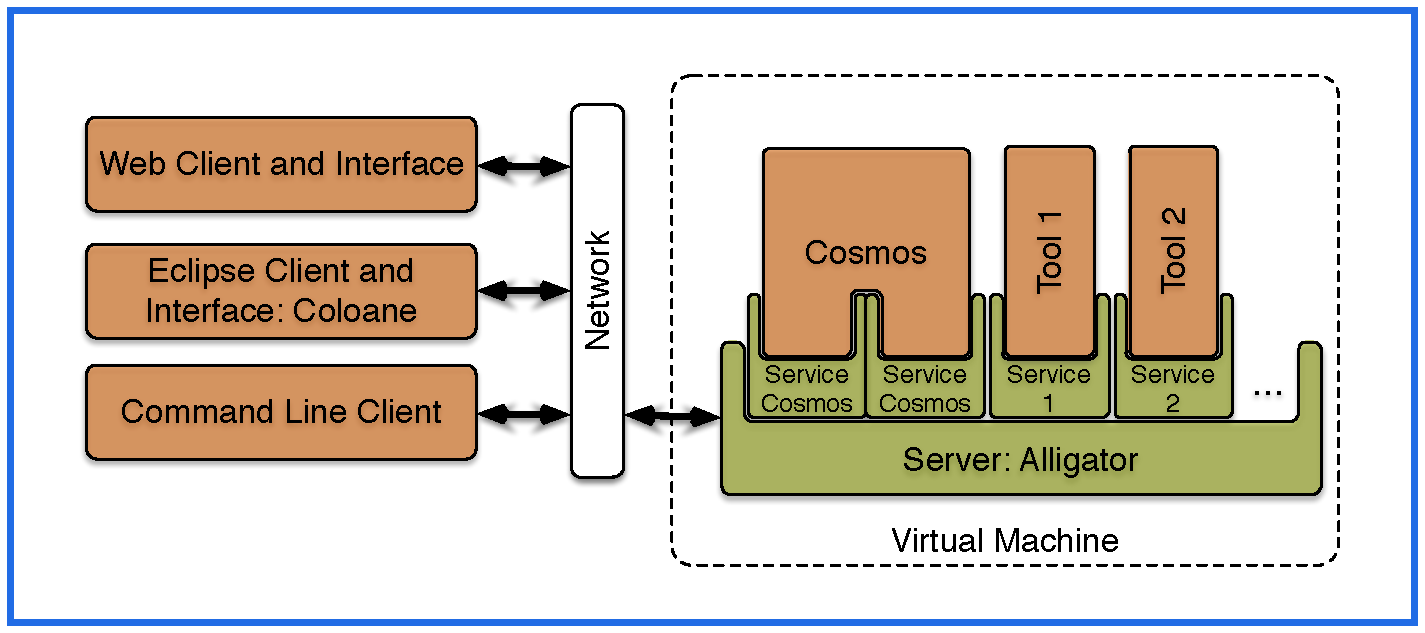
\includegraphics[scale=0.50]{img/cosyverif_schema.pdf}
    \\
    \hfill{Source: Benoît Barbot}
    \caption{Architecture de CosyVerif}
\end{figure}

La plateforme CosyVerif a été conçue de manière à :
\begin{itemize}
\item manipuler des formalismes différents avec la possibilité de créer facilement de nouveaux,
\item fournir une interface graphique pour chaque formalisme permettant l'édition de modèles,
\item inclure des outils de vérification appelées via l'interface en tant
  que services web,
\item offrir la possibilité pour un développeur d'intégrer son propre outil,
  en lui permettant d'interagir avec les autres outils.
\end{itemize}

Deux familles de formalismes sont actuellement pris en charge: les automates
et les réseaux de Petri. Pour chaque famille, plusieurs formalismes sont
disponibles (réseaux P/T, colorés, stochastiques, ...).
La plupart des outils manipulent pour l'instant des réseaux de Petri. Certains d'entre eux procèdent à des analyses structurelles comme 
des calculs d'invariants, tandis que d'autres effectuent des analyses
comportementales, comme la construction de graphe 
d'accessibilité.
Tous les logiciels développés sont sous licences libres, mais certains
outils peuvent ne pas l'être, comme par exemple GreatSPN.

\subsection{Problèmes identifiés}

Les choix techniques pour la réalisation de la plateforme ont jusqu'ici été
influencés par les composants pré-existants. La première brique fut Coloane,
écrit en Java sous la forme d'une plug-in Eclipse.

Le serveur a donc été lui aussi développé en Java, afin de conserver un seul
langage.
Le protocole SOAP a été choisi comme protocole de communication entre les
deux,
car il dispose d'une excellente interface Java, ne nécessitant qu'un minimum
de développement.

\medskip

Plusieurs problèmes ont mené à la redéfinition technique du projet
CosyVerif.

Premièrement, le client graphique actuel, Coloane, n'est plus maintenable, car aucun
membre permanent du projet ne maîtrise le développement de plug-in Eclipse.

Deuxièmement, il est apparu que l'utilisation de SOAP n'est pas
pratique hors du monde Java, ce qui crée un fort couplage entre le serveur et ses clients.
De plus, l'environnement Java, ainsi que la surcouche et le moteur de SOAP
ajoutent de très nombreuses dépendances transitives, qui pèsent plusieurs dizaines de méga-octets.
Troisièmement, le serveur a posé des problèmes de confinement. En effet, les
outils étant directement lancés par le serveur, il est arrivé qu'ils fassent
planter la Java Virtual Machine, et donc le serveur complet.
Un confinement a été mis en place, mais il est très coûteux en ressources
(temps et mémoire).

Quatrièmement, l'ajout de nouvelles fonctionnalités simples au serveur,
telles que l'authentification, s'est avérée plus complexe que prévu. En
effet, les bibliothèques utilisées nécessitent un apprentissage conséquent
pour de telles choses.

Ces problèmes de la plate-forme existante ont conduits l'équipe à repartir sur une nouvelle base, 
tout en restant vigilant pour ne pas retomber sur les mêmes difficultés.
Pour ces raisons, l'équipe a émis des exigences assez fortes pour 
la nouvelle plate-forme.

\section{Sujet du stage}

L'objectif de mon stage est de concevoir et développer le nouveau serveur de
la plateforme CosyVerif. Cet objectif a été étendu au cours du stage au
client web de la plate-forme.

Le nouveau serveur dispose de fonctionnalités nouvelles par rapport au
serveur existant : dépôt de modèles et de formalismes, éditions
collaborative de modèles, authentification des utilisateurs.
Il intègre aussi les fonctionnalités déjà existantes : la gestion
d'exécution d'outils.

\subsection{Que doit offrir la future plate-forme ?}

La plate-forme doit permettre :

\begin{itemize}
\item la recherche de formalismes et de modèles selon certains critères,
\item l'insertion des nouveaux formalismes et modèles et leur édition,
\item l'authentification des utilisateurs,
\item la gestion de permissions des utilisateurs,
\item l'insertion de nouveaux outils,
\item l'exécution d'outils.
\end{itemize}

\subsection{Exigences de l'encadrement}

Les exigences à prendre en compte, qui ont été imposées par l'équipe, pour
réaliser la nouvelle plate-forme, sont :

\begin{itemize}
\item les tests doivent être effectuées en boîte noire avec une couvertir complète du code,
\item le code doit être maintenable et simple,
\item le code source doit être écrit et commenté en anglais,
  les commentaires seront rédigés en programmation lettrée,
\item seules des technologies simples et légères seront utilisées;
  des technologies lourdes telles que SOAP ou Eclipse sont interdites.
\end{itemize}

\subsection{Axes de ma contribution sur la future plate-forme}

\paragraph{}
La nouvelle plate-forme présente 5 composants distincts qui sont étudiés et réalisés séparément et intégrés par la suite : trois composants côté serveur et deux autres côté client web.
J'ai réalisé deux de ces composants au cours de mon stage. Un autre a été
réalisé par un autre stagiaire (Francisco Gimenez), et le reste par
l'ingénieur du projet.

\subsubsection{Côté serveur}

\begin{itemize}
\item Dépôt : ce composant est chargé du dépôt de modèles et de formalismes, de la gestion d'authentifications 
et de droits d'accès des utilisateurs.
\item Édition : ce composant s'occupe de l'édition collaborative de modèles et de formalismes. Il interagit 
directement avec le composant édition web du client au moment de l'édition
collaborative,
ainsi qu'avec le dépôt.
\item Exécution : ce composant s'occupe de l'exécution d'outils. Il n'est à ce
  jour pas complètement défini.
\end{itemize}

\subsubsection{Côté client}

\begin{itemize}
\item Interface web : ce composant est l'interface web qu'un utilisateur a pour s'authentifier auprès du serveur, pour utiliser le dépôt de modèles et de formalismes, pour participer à des projets avec d'autres utilisateurs, pour lancer des outils et observer leurs résultats. C'est le composant du client qui communique et échange des données avec le serveur dépôt.
\item Editeur web : Ce composant est l'interface web qui permet l'édition de modèles et de formalismes. C'est le composant du client qui interagit directement avec le composant serveur d'édition.
\end{itemize}

L'interaction entre ces composants est schématisé dans la
figure~\ref{fig:interaction}.
\begin{figure}[h!]
    \centering
    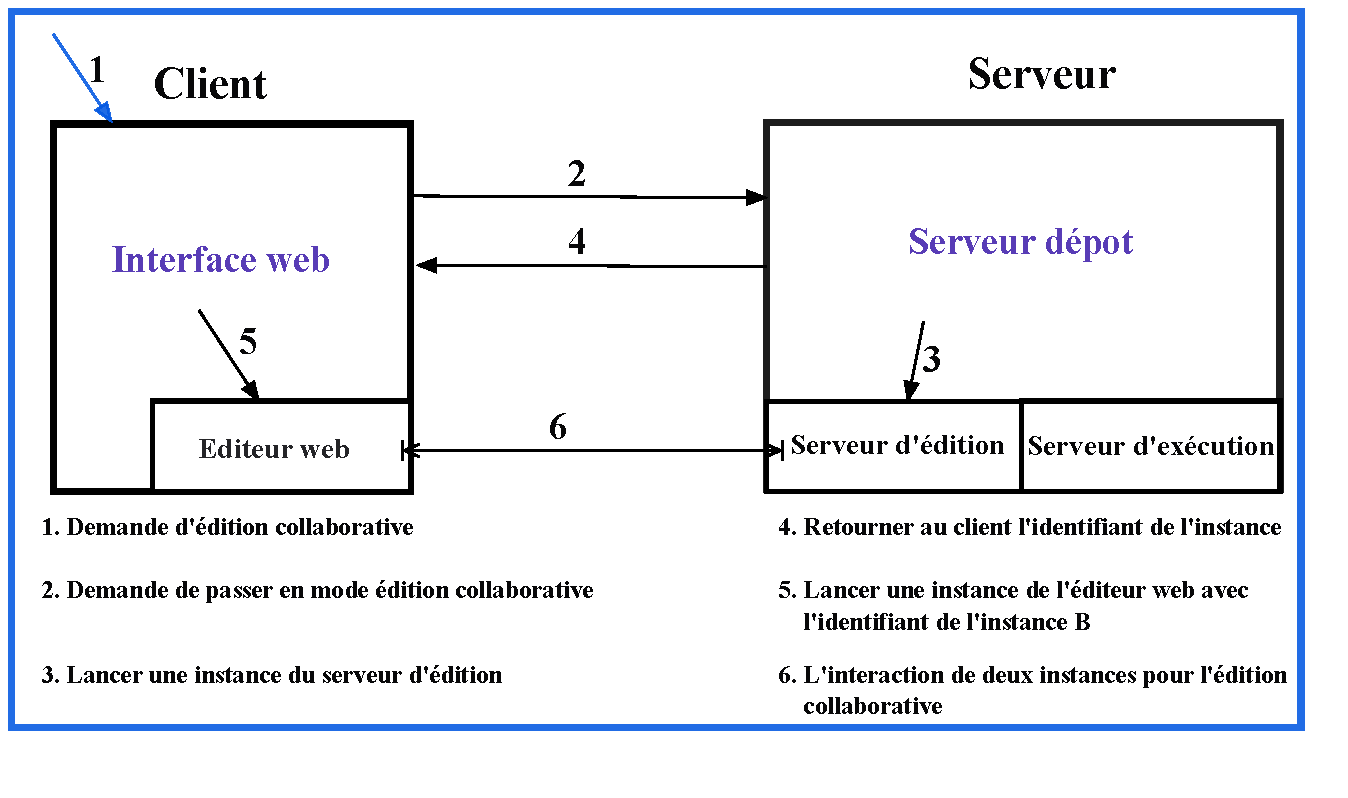
\includegraphics[scale=0.60]{img/cosyverif_composants.pdf}
    \caption{Exemple d'interactions entre les différents composants (édition collaborative)}
    \label{fig:interaction}
\end{figure}

\medskip

Mon stage consiste à concevoir et à réaliser le serveur de dépôt. Il a été
étendu pour réaliser l'interface web du client. Les serveurs d'édition et
d'exécution sont réalisés par Alban Linard (encadrent) et l'éditeur web par
Francisco Gimenez (un autre stagiaire).



%%%%%%%%%%%%%%%%%%%%%%%%%%%%%%%%%%%%%%%%%%%%%%%%%%%%%%%%%%%%%%%%%%%%%%%%%%%%%%%%
%%%%%%%%%%%%%%%%%%%%%%%%%%%%%%%%%%%%%%%%%%%%%%%%%%%%%%%%%%%%%%%%%%%%%%%%%%%%%%%%

\chapter{Conception et réalisations du serveur}

Le dépôt est le composant centrale du serveur de la plate-forme CosyVerif. D'une part, il est chargé de la
gestion de comptes utilisateurs et du dépôt de modèles et de formalismes de
la plate-forme. D'autre part, c'est le composant  qui satisfait toute les
requêtes de l'interface des clients (mis à part l'édition 
collaborative et de l'exécution d'outils) et qui est initiateur de l'édition collaborative et de l'exécution d'outils.
Les clients attendus sont : web, téléphone mobile, console et des bibliothèques.

Le serveur définit des
ressources, et des méthodes d'accès (création, lecture, écriture,
suppression) sur ces ressources. Il est sans état, c'est-à-dire
qu'il ne maintient aucun état de connexion avec les clients.

\section{Ressources}

Le dépôt de la plate-forme contient des ressources, parmi un ensemble
prédéfini :
\begin{itemize}
  \item utilisateurs,
  \item projets,
  \item formalismes,
  \item modèles,
  \item convertisseurs,
  \item services,
  \item exécutions,
  \item scénarios.
\end{itemize}

Les ressources présentes dans le dépôt appartiennent aux utilisateurs.
Les ressources peuvent être publiques ou privées.
Par conséquent, il faut un système capable d'identifier
les utilisateurs et de vérifier leurs droits correspondants à l'utilisation d'une ressource. A cet effet, un système 
d'organisation et de protection des ressources a été réalisé.

\subsection{Organisation de ressources}

Un des objectifs pour la plate-forme CosyVerif est de mettre à disposition de ses utilisateurs un moyen pour permettre
d'avoir des ressources propres et de partager des ressources entre utilisateurs.

\subsubsection{Ressources propres}
Pour permettre aux utilisateurs d'avoir ses propres ressources, chaque
utilisateur a un compte à sa disposition. Un utilisateur peut y créer des ressources, les utiliser et les mettre à jour mais aussi permettre à 
d'autres utilisateurs d'y accéder.
Cependant, on ne peut accéder aux ressources d'un autre utilisateur qu'en
lecture seule, sans les modifier.

La visibilité du compte d'un utilisateur, et donc des ressources contenues,
est globalement publique ou privée.
Un compte publique donne droit de lecture de ses ressources à tout 
utilisateur et un compte privé ne donne ce droit qu'au propriétaire du compte.

Ce système de droits est extrêmement simple, mais il ne permet pas de
couvrir tous les cas d'utilisation. Par exemple, avec ce système, il est
impossible à deux utilisateurs de travailler (en écriture) sur le même
modèle. Il leur est aussi impossible d'accéder tous deux à un modèle privé.

\subsubsection{Ressources partagées}
Tout utilisateur de la plateforme peut décider de créer un projet. Celui-ci
est similaire à un compte utilisateur, et contient ses propres ressources.
Cependant, il est possible d'inviter ou d'ajouter d'autres utilisateurs à
projet, ce qui permet de travailler à plusieurs sur les même ressources.

Quand, un utilisateur
désire de partager des ressources avec un ou plusieurs utilisateurs, il crée un projet et invite les autres à y joindre (ou 
les autres font eux mêmes la demande).

Un projet peut être public ou privé, comme un compte utilisateur,
ce qui permet d'avoir des projets accessibles à tous en lecture, ou bien
limités à certains utilisateurs.


\subsection{Protection des ressources}
La plate-forme de CosyVerif est une plate-forme publique et peut être accéder par n'importe qui, à partir du moment où
l'on a l'accès à Internet.
Cependant, certaines ressources, celles situées dans des comptes utilisateurs ou
projets privés, ne doivent pas être lisible de tous. De même, les ressources
d'un utilisateur ne doivent être modifiables que par lui-même.

Pour répondre 
à ce besoin de protection des ressources, le serveur met en place une
politique de sécurité basée sur un système d'authentification et un système
d'autorisation des utilisateurs.
Afin de garantir le caractère privé des données, on utilise aussi un système
de chiffrement des données échangées entre les clients et le serveur : SSL.

\subsubsection{Système d'authentification}
Les ressources de la plate-forme sont utilisées par deux catégories d'utilisateurs : 
\begin{itemize}
\item Des utilisateurs authentifiés : ce sont des utilisateurs muni d'un login et d'un mot de passe qui font des requêtes au 
serveur et qui sont identifiés par ce dernier. Cette catégorie
d'utilisateurs peut créer et utiliser ses propres ressources et
accéder en lecture à toutes les ressources publiques.
\item Des utilisateurs non authentifiés : ce sont des utilisateurs qui font des requêtes au serveur sans présenter de login 
et de mot de passe. Cette catégorie d'utilisateurs ne peut qu'accéder en
lecture aux ressources publiques.
\end{itemize}

La plate-forme disposant de la notion de compte utilisateur, un système d'authentification est mis en place. Ce dernier identifie les utilisateurs à l'aide d'un login et d'un mot de passe. Cependant, il y a des précautions à prendre pour éviter certaines 
failles. Différentes techniques existent pour sécuriser les échanges de la plate-forme :

\begin{quotation}
  \noindent
\begin{itemize}
\item Hachage de mot de passe : d'une part, il permet de ne pas faire circuler le mot de passe clairement sur le réseau et 
d'autre part, il permet également de ne pas stocker le mot de passe de l’utilisateur en clair. Cependant, le mot de passe ainsi haché peut être retrouvé dans certains cas
\item Utilisation d’un "salt" : même s'il est à priori impossible de retrouver le mot de passe à partir du hash, de 
nombreux dictionnaires de conversion existent sur internet faisant le rapprochement entre un hash et un mot de passe.
Une solution de contournement est l'utilisation d'un "salt" qui est une technique qui consiste à hasher une première fois 
le mot de passe, à concaténer le hash à une chaîne de caractère (salt) et à le hasher une seconde fois. Le salt est unique 
et connu à la fois du serveur et de l’application cliente, il n’est pas caché au yeux du hacker. Son seul but est de rendre 
votre mot de passe indéchiffrable sur le réseau. Cependant, dans le cas où un hacker arrive à intercepter le mot de passe encrypté, il aura tout le temps qu’il souhaite pour exécuter n’importe quelle requête en notre nom.
\item Token d’authentification : l’idée du token d’authentification est simple. Celle-ci consiste à envoyer dans un 1er temps un couple login/password et de récupérer un token en retour. Dans un second temps, ce token devra être utilisé 
à la place du password. Ceci permet, coté serveur, de gérer la durée de validité des tokens (à 20 minutes par exemple). 
Cependant, dans le cas où un hacker arrive à intercepter notre token d’authentification, il aura une vingtaine de 
minutes pour exécuter n’importe quelle requête en notre nom. l’utilisation du token ne permet, du point de vue de l’utilisateur, que de se substituer au password. Il ne certifie en aucun cas que vous êtes l’émetteur de la requête. La technique consiste alors à remplacer notre token d’authentification par une signature sur la requête. 
\item Signer ses requêtes : Le principe des signatures est d’ajouter un paramètre supplémentaire à notre requête afin de
garantir au récepteur à la fois l’identité du rédacteur de la requête ainsi que l’intégrité de celle-ci. Avec cette signature, 
même si un hacker parvient à récupérer notre requête, la seule action qu’il sera en mesure de réaliser sera de rejouer 
cette même requête sans y changer aucun paramètre. Cependant, c'est aussi un problème.
\item  Requêtes à usage unique : Ce type de requête est utilisée par la plupart des fournisseurs tels qu’Amazon Web 
Services. La technique est simple, il suffit d’ajouter le timestamp à la signature ainsi qu’aux paramètres de la requête lors 
de la génération de la requête. Ainsi, le serveur n’a qu’à stocker le timestamp de la dernière requête traitée et le 
comparer avec celui de la requête en cours. Si le timestamp de la requête courante est inférieur ou égal à celui du dernier 
timestamp enregistré, cela signifie que la requête à déjà été jouée. Sinon, cela signifie que la requête est jouée pour la 
1ere fois. Cependant, même si votre requête ne peut être ni altérée ni rejouée, celle-ci peut être « vue » par un hacker. Dans la plupart des cas, ceci n’a que peu d’importance mais dans le cadre d’une application bancaire, il est n’est pas envisageable qu’une tiers personne puisse connaître les montants et les destinataires de vos virements.
\item  SSL : SSL (pour Secure Socket Layer) est un système permettant de sécuriser les échanges de données entre deux 
ordinateurs. Associés par exemple, le HTTP et le SSL donnent le HTTPS. Ce protocole est intégré à l’immense majorité des 
navigateurs web et permet de sécuriser les échanges entre l’utilisateur et le serveur. En utilisant du HTTPS, vous pouvez 
être sûr que personne n’interceptera vos requêtes. Ce mécanisme vous assure la sécurité du transport et uniquement de 
celui-ci (pas de gestion d’authentification, d’unicité des requêtes, …).
\end{itemize}
\end{quotation}
\hfill{Source: \url{http://blog.ineat-conseil.fr/2013/01/restful-authentication/}}

\medskip

Par soucis de simplicité, à la fois du serveur et des clients, le choix a été porté sur un système d'authentification basique basé sur la combinaison de la technique de hachage de 
mot de passe et le protocole SSL. Ce choix va permettre de sécuriser les mots de passes présents dans le système de
stockage du serveur dans le cas où un pirate parviendrait à les récupérer et, aussi de rendre la requête illisible par les 
éventuels pirate qui récupéreraient cette requête sur internet. Nous avons fait ce choix car CosyVerif n'est pas un système
critique et ne présente d'autre danger que la circulation en claire du mot de passe
(pour l'instant).

L'authentification se déroule de la manière suivante. Puisque le serveur est
sans état, à chaque requête, l'utilisateur présente un login et un mot de passe auprès du serveur.
Ce dernier vérifie l'identité de l'utilisateur dans son annuaire d'utilisateurs. S'il réussit à identifier l'utilisateur, il lui donne l'accès à 
ses ressources. Sinon, il lui refuse l'accès. Cependant, La phase d'authentification ne garantie pas la satisfaction de toutes 
les requêtes de l'utilisateur. Il faut aussi une autorisation pour utiliser les ressources sollicitées.

\subsubsection{Système d'autorisation}
Le serveur, même s'il arrive à identifier un utilisateur, ne lui donne pas
tous les droits d'accès sur les ressources.
Le serveur associe des droits d'utilisation à ses ressources, tels que le droit de création, de lecture, de mise à jour et de 
suppression de ressource, mais aussi le droit d'administration d'un compte utilisateur ou d'un projet. Une étude a été faite
sur deux stratégies :
\begin{itemize}
\item Droits associés à chaque ressource : chaque ressource dispose d'une
  liste d'utilisateurs avec leurs droits associés. Cette stratégie permet
  alors à un utilisateur de donner finement des droits sur chacune de ses
  ressources, de manière individuelle.
  Dans ce cas, la notion de projet est redondante pour partager des ressources avec d'autres
utilisateurs. Cette stratégie n'est pas difficile à mettre en oeuvre mais
nécessite beaucoup d'effort de la part 
des utilisateurs. En effet, ce système est complexe à utiliser car il faut une gestion
de droits d'utilisation sur chaque ressource. Cette stratégie est à éviter
car la plate-forme CosyVerif a pour vocation d'être la plus simple possible
d'utilisation.
\item Droits associés aux comptes utilisateurs et aux projets : dans cette stratégie, les ressources d'un utilisateur sont
soit toutes publiques, soit toutes privées.
Les ressources d'un utilisateur ne sont modifiable que par lui-même, ou dans
le cadre d'un projet, par les autres membres du projet.
Si un utilisateur décide de partager des ressources, il crée un projet,
déplace les ressources dans celui-ci, et invite d'autres utilisateurs à se joindre au projet.
Les membres d'un projet ont différents droits : lecture, écriture ou
administration.
\end{itemize} 

La seconde stratégie est adoptée pour le système d'autorisation car elle nécessite peu
d'effort de la part des utilisateurs.


La liste de droits d'utilisation de la solution retenue est donnée
ci-dessous :

\begin{itemize}
\item Propriétaire d'un compte : un utilisateur a tous les droits sur son compte et sur ses ressources,
\item Droit d'administration des comptes utilisateurs : ce droit est donné à un utilisateur pour créer, mettre à jour ou
supprimer un compte utilisateur quelconque,
\item Compte utilisateur public : un compte utilisateur publique donne le droit de lecture de ses ressources à tous les
utilisateurs de la plate-forme,
\item Compte utilisateur privé : un compte utilisateur privé ne donne aucune droit d'utilisation à d'autres utilisateurs que
son propriétaire,
\item Participants d'un projet : tous les utilisateurs qui participent à un projet ont le droit de lecture.
\item Droit d'administration d'un projet : ce droit est donné à un utilisateur d'un projet pour mettre à jour le projet, 
supprimer un utilisateur du projet et inviter, accepter ou refuser des utilisateurs au projet.
\item Droit d'édition d'un projet : ce droit est donné à un utilisateur d'un projet pour créer, lire, modifier et supprimer 
des ressources du projet.
\item Projet public : un projet publique donne le droit de lecture de ses ressources à tous les utilisateurs de la 
plate-forme,
\item Projet privé : un projet privé ne donne aucune droit d'utilisation à d'autres que les utilisateurs qui y
participent,
\end{itemize}

% -- Tableau 1 compte user : URIs,  propriétaire,  autre utilisateur authentifié sans droit admin,  autre utilisateur authentifié avec droit admin, autre utilisateur non authentifié


% -- Tableau 2 projet : URIs, Participant sans droit, Participant avec droit admin, Participant avec droit d'édition, Non participant



\section{Définition de l'architecture et du protocole}
\paragraph{}
Le nouveau serveur doit être une application REST (Representational State Transfer) ou RESTful. RESTful est un style
d’architecture permettant de construire des applications (Web, Intranet, Web Service, surtout pour les systèmes 
hypermédia distribués). Il s’agit d’un ensemble de conventions et de bonnes pratiques à respecter et non d’une 
technologie à part entière. L’architecture REST utilise les spécifications originelles du protocole HTTP, plutôt que de
réinventer une surcouche (comme le font SOAP ou XML-RPC par exemple).

\paragraph{}
La communication du serveur avec les clients se base sur : 
\begin{itemize}
\item Des requêtes HTTP,
\item Des URLs pour les ressources,
\item Les verbes HTTP (GET, POST, ...) pour les méthodes,
\item Les codes d'état pour les résultats,
\item Les contenus des requêtes et des résultats 
\end{itemize}

Les contraintes
d'une architecture REST sont les suivantes :
\begin{quotation}
  \noindent
\begin{enumerate}
\item Client-serveur : les responsabilités sont séparées entre le client et le serveur. L'interface utilisateur est séparée de
celle du stockage des données. Cela permet aux deux d'évoluer indépendamment ;
\item Sans état : chaque requête d'un client vers un serveur doit contenir toute l'information nécessaire pour permettre 
au serveur de comprendre la requête, sans avoir à dépendre d'un contexte conservé sur le serveur. Cela libère de 
nombreuses interactions entre le client et le serveur ;
\item Une interface uniforme : cette contrainte agit selon 4 règles essentielles :
    \begin{itemize}
    \item L'identification des ressources : chaque ressource est identifiée uniquement,
    \item La manipulation des ressources à travers des représentations : les ressources ont des représentations définies,
    \item Un message auto-descriptif : les messages expliquent leur nature. Par exemple, si une représentation en HTML 
    est codée en UTF-8, le message contient l'information nécessaire pour dire que c'est le cas,
    \item Hypermédia comme moteur d'état de l'application : chaque accès aux états suivants de l'application est décrit 
     dans le message courant
    \end{itemize}
\item Mise en cache : le serveur envoie une réponse qui donne l'information sur la propension de cette réponse à être mise en cache, comme la fraîcheur, sa date de création, si elle doit être conservée dans le futur. Cela permet à des
serveurs mandataires de décharger les contraintes sur le serveur et aux clients de ne pas faire de requêtes inutiles. Cela
permet également d'améliorer l'extensibilité des serveurs ;
\item Un système hiérarchisé par couche : les états de l'application sont identifiées par des ressources individuelles. 
Toute l'information n'est pas envoyée dans une seule ressource unique. Les requêtes/réponses entre le client et le 
serveur augmentent et donc peuvent faire baisser la performance d'où l'importance de la mise en cache, etc. Le bénéfice
est que cela rend beaucoup plus flexible l'évolution du système.
\end{enumerate}

\paragraph{}
La thèse de Roy Fielding précise les avantages de ce style architectural par rapport à d’autres styles d’architectures 
d’applications Web. Citons entre autres :

\begin{enumerate}
\item L’application est plus simple à entretenir, car elle désolidarise la partie client de la partie serveur. La nature 
hypermédia de l'application permet d'accéder aux états suivants de l'application par inspection de la ressource courante;
\item L'absence de gestion d’état du client sur le serveur conduit à une plus grande indépendance entre le client et le 
serveur. Elle permet également de ne pas avoir à maintenir une connexion permanente entre le client et le serveur. 
Le serveur peut ainsi répondre à d'autres requêtes venant d'autres clients sans saturer l'ensemble de ses ports de 
communication. Cela devient essentiel dans un système distribué;
\item L’absence de gestion d’état du client sur le serveur permet également une répartition des requêtes sur plusieurs 
serveurs : une session client n’est pas à maintenir sur un serveur en particulier (via une sticky session d’un loadbalancer), ou à propager sur tous les serveurs (avec des problématiques de fraîcheur de session). Cela permet aussi une meilleure 
évolutivitée et tolérance aux pannes (un serveur peut être ajouté facilement pour augmenter la capacité de traitement, ou pour en remplacer un autre);
\item Dans un contexte Web
    \begin{itemize}
    \item l’utilisation du protocole HTTP en tirant parti de son enveloppe et ses en-têtes,
    \item l’utilisation d’URI comme représentant d’une ressource permet d'avoir un système universel d'identification des 
     éléments de l'application,
    \item la nature auto-descriptive du message permet la mise en place de serveurs cache. Les informations nécessaires
     sur la fraîcheur, la péremption de la ressource sont contenues dans le message lui-même
    \end{itemize}
\end{enumerate}
\end{quotation}
\hfill{Source : \url{http://fr.wikipedia.org/wiki/Representational_State_Transfer}}

\medskip

Pour répondre aux contraintes de REST, nous avons définit : 
\begin{itemize}
\item les ressources, leurs contenus et leurs représentations,
\item les méthodes prises en charge, les entrées, les sorties et les codes d'état.
\end{itemize}

\subsection{URIs}
\paragraph{}
Le serveur utilise les ressources suivantes : 

\begin{itemize}
    \item users,
    \item formalisms,
    \item models,
    \item converters,
    \item scenarios,
    \item services,
    \item executions,
    \item projects.
\end{itemize}

Pour identifier les ressources, REST utilise des Uniform Ressource Identifiers (URIs). Un client demande une ressource au 
serveur en lui fournissant l'URI de la ressource. Il existe deux types de ressources dans cette application : \\
\begin{itemize}
  \item des collections de ressources (users, models, ...),
    \item des ressources simples (model, user, ...).
\end{itemize}

Les deux types se distinguent par l'utilisation de la forme singulière (pour les ressources individuelles) ou au pluriel (pour les
collections de ressources).

Par exemple : 
\begin{itemize}
  \item \lstinline!/users/! représente la collection des utilisateurs;
    \item \lstinline!/users/rokysaroi! représente l'utilisateur rokysaroi dans la collection d'utilisateur.
\end{itemize}

Les figures \ref{fig:hierarchy} et \ref{fig:uri} montrent la hiérarchie des ressources.
Un nom de ressource à partir de ":" par exemple ":user", est une variable. La liste suivante montre également les URIs des
ressources. La notation (a|b) indique qu'une ressource est disponible pour les préfixes a et b.


\begin{figure}[h!]
     \centering
     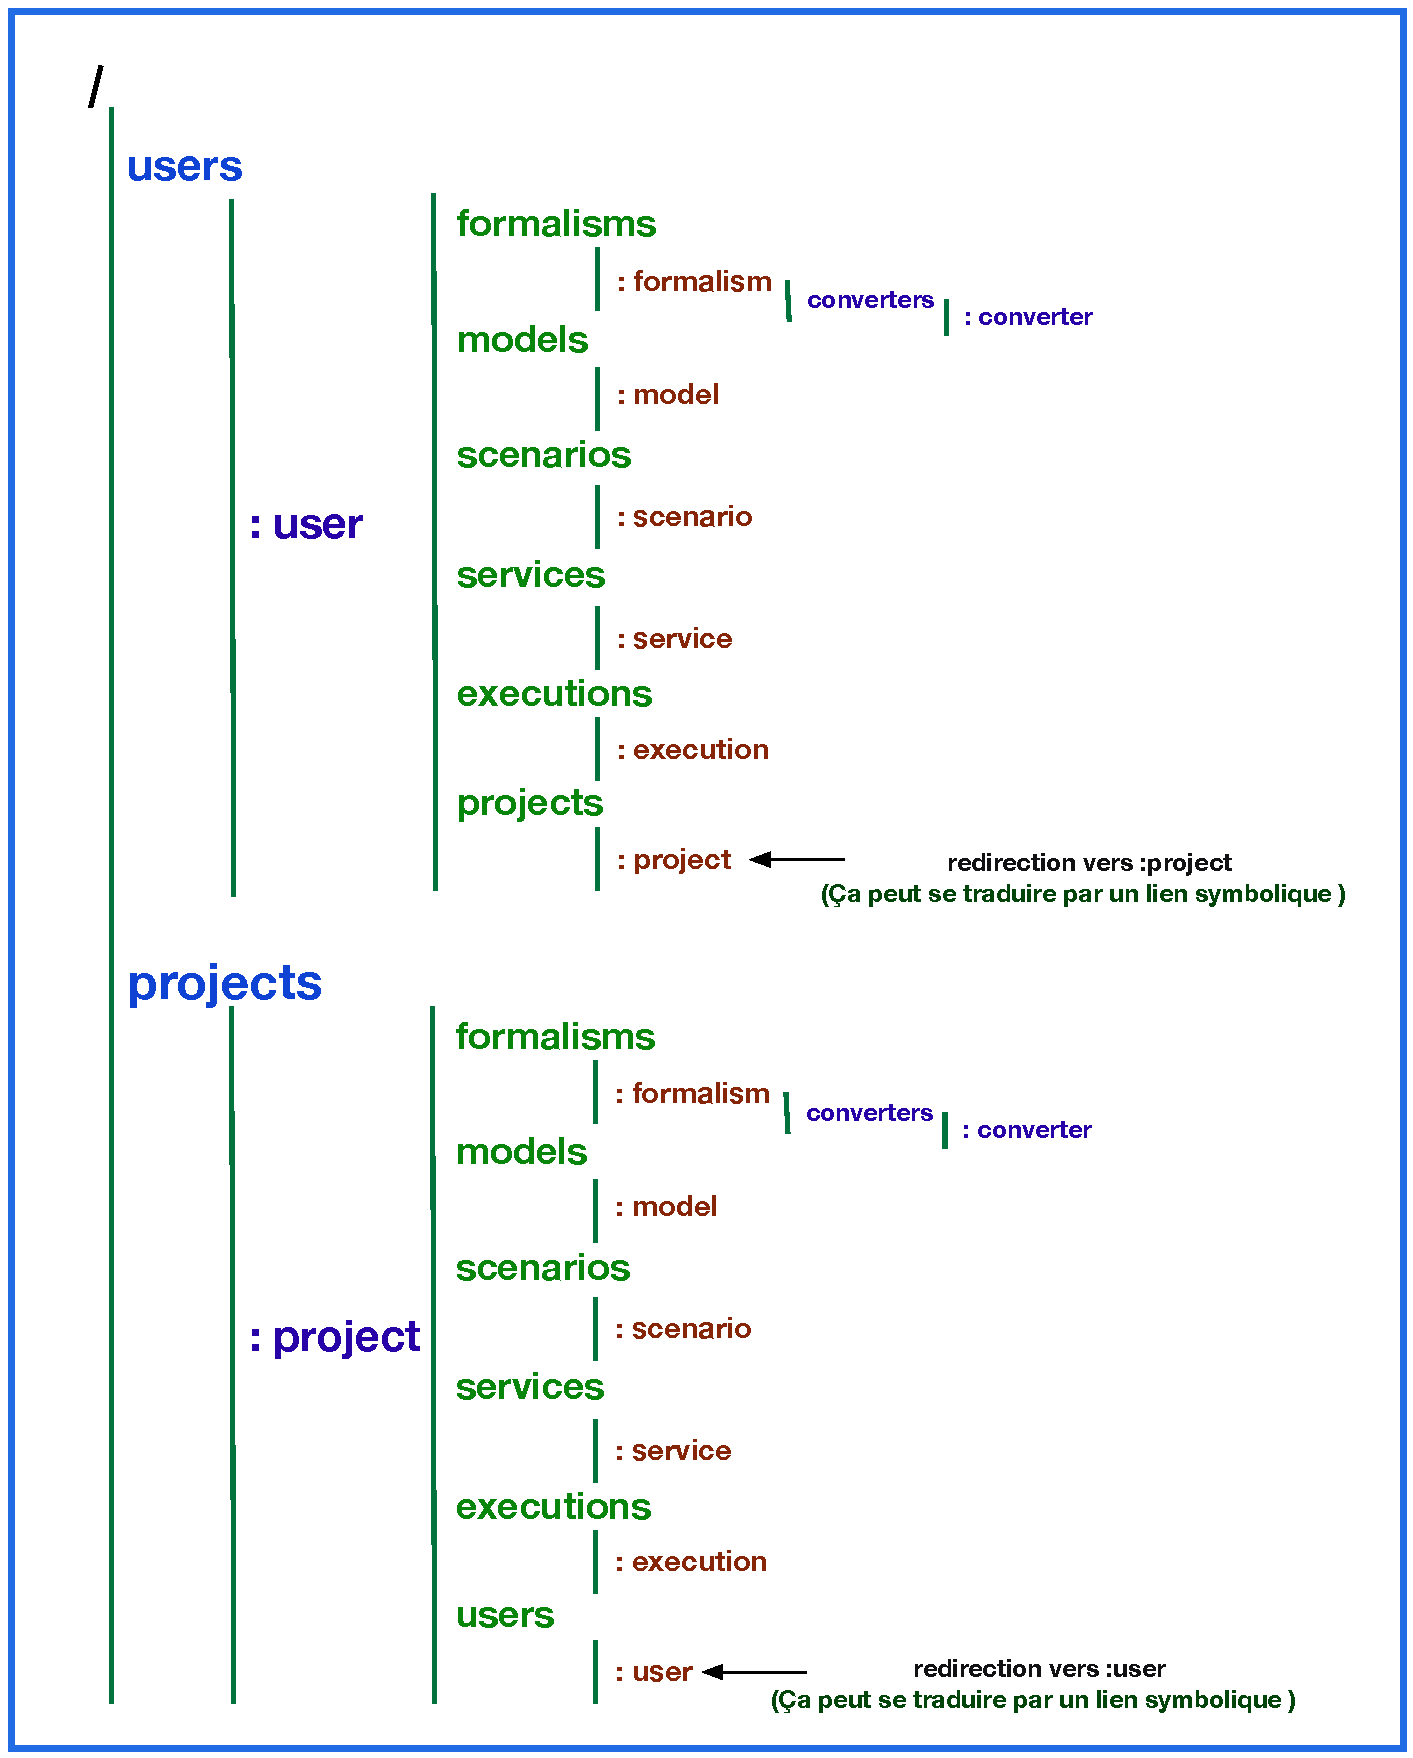
\includegraphics[scale=0.60] {img/resources_hierarchy.pdf}
     \caption{Hiérarchie des ressources}
     \label{fig:hierarchy}
\end{figure}

\begin{figure}[h!]
    \centering
    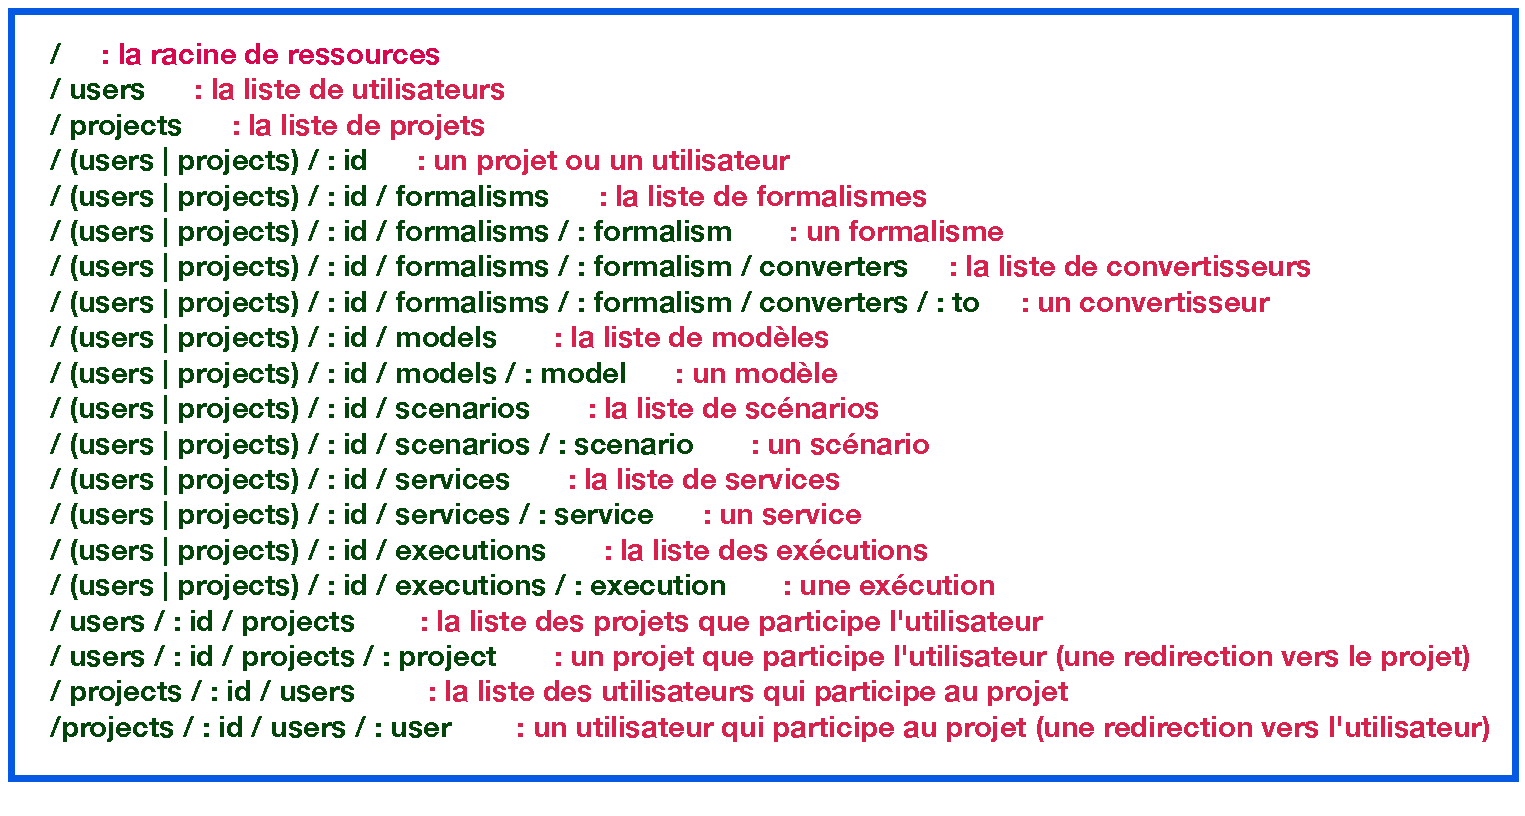
\includegraphics[scale=0.60]{img/resources_uri.pdf}
    \caption{Hiérarchie des ressources}
    \label{fig:uri}
\end{figure}

\subsection{Représentation de ressources}

\paragraph{}
Une ressource peut avoir plusieurs représentations (XML, JSON, image, le format CosyVerif, CAMI, PNML, ...). En interne, 
le serveur utilise la représentation CosyVerif pour les ressources suivantes : formalisme, modèle, scénario, service, 
exécution, et le format JSON pour les autres.

Les clients sont autorisés à demander une représentation particulière dans leurs requêtes. Lorsque cela est possible, le 
serveur effectue une conversion de la ressource à la forme requise : des convertisseurs sont prévus pour ça.
La notion de convertisseurs est prévue pour cela, permettant par exemple de
convertir un modèle en PNML. Cependant, cette notion n'est pour l'instant
pas étudiée dans le cadre du projet CosyVerif.

      
\subsection{Méthodes et codes de statut}

\paragraph{}
L'architecture REST est basé sur le protocole HTTP. Par conséquent, les mêmes méthodes sont plus ou moins utilisées. 
Le protocole est normalisé. Les clients utilisent une URI pour accéder à une 
ressource référencée. L'accès peut prendre diverses formes, telles que l'obtention d'une représentation de la ressource 
(par exemple, en utilisant la méthode GET ou la méthode HEAD), l'ajout ou la modification d'une ressource (par exemple, 
en utilisant la méthode POST ou la méthode PUT) et la suppression d'une ressource (par exemple, via la méthode DELETE).

\paragraph{}
Les méthodes suivantes seront intégrées dans le système :

\begin{itemize}
   \item POST : création une ressource,
   \item GET : récupération d'une ressource,
   \item PUT : mise à jour d'une ressource,
   \item PATCH : mise à jour partielle d'une ressource,
   \item DELETE : suppression d'une ressource.
\end{itemize}

\paragraph{}
Chaque réponse HTTP contient un code (code de statut). Ce code est utilisé par le serveur pour informer le client de l'état 
du traitement de sa demande. Le code d'état est un code numérique et une description donnant une réponse 
humainement compréhensible. 

\paragraph{}
Les codes de retours suivants sont utilisables dans CosyVerif.
Ces codes de statuts sont une partie de ceux spécifiés par la norme RFC 2616.
\begin{quotation}
\begin{tabular}{|p{1cm}|p{4cm}|p{9cm}|}
\hline \bf Code & \bf Message & \bf Signification \\
\hline 200 & OK & Requête traitée avec succès \\
\hline 201 & Created & Requête traitée avec succès avec création d’un document \\
\hline 204 & No Content & Requête traitée avec succès mais pas d’information à renvoyer \\
\hline 301 & Moved Permanently & La ressource demandée possède une nouvelle adresse (URI). Toute référence future à cette ressource doit être faite en utilisant l'une des URIs retournées dans la réponse. Le client doit normalement charger 
automatiquement la ressource demandée à sa nouvelle adresse. \\
\hline 302 & Moved Temporarily & La ressource demandée réside temporairement à une adresse (URI) différente. Cette 
redirection étant temporaire, le client doit continuer à utiliser l'URI originale pour les requêtes futures \\
\hline 400 & Bad Request & La syntaxe de la requête est erronée \\
\hline 401 & Unauthorized & Une authentification est nécessaire pour accéder à la ressource \\
\hline 403 & Forbidden & Le serveur a compris la requête, mais refuse de l’exécuter. Contrairement à l’erreur 401, 
s’authentifier ne fera aucune différence. Sur les serveurs où l’authentification est requise, cela signifie généralement que 
l’authentification a été acceptée mais que les droits d’accès ne permettent pas au client d’accéder à la ressource \\
\hline 404 & Not Found & Ressource non trouvée \\
\hline 405 & Method Not Allowed & Méthode de requête non autorisée \\
\hline 410 & Gone & La ressource est indisponible et aucune adresse de redirection n’est connue. Ce code sera utilisé 
pour les ressources supprimées ; on mettra une information à la place d’une ressource supprimée. \\
\hline 415 & Unsupported Media Type & Format de requête non supporté pour une méthode et une ressource données \\
\hline 422 & Unprocessable entity & L’entité fournie avec la requête est incompréhensible ou incomplète \\
\hline 500 & Internal Server Error & Erreur interne du serveur \\
\hline 501 & Not Implemented & Fonctionnalité réclamée non supportée par le serveur \\
\hline
\end{tabular}
\end{quotation}
\hfill{Source : \url{http://fr.wikipedia.org/wiki/Liste_des_codes_HTTP}}

\medskip

Pour un type de ressource, tous les codes de statuts ne peuvent pas être
retournés. Le tableau ci-dessous précise quels codes sont utilisés pour les
différents types de ressources.

\begin{tabular}{|p{3cm}|p{2cm}|p{3cm}|p{6cm}|}
\hline \bf Ressource & \bf Méthode & \bf Representation & \bf Codes de statuts \\
\hline Utilisateur & GET & Format user & 200, 400, 401, 403, 404, 410, 415, 500 \\
\hline Utilisateur & PUT & Format user & 200, 201, 400, 401, 403, 415, 500 \\
\hline Utilisateur & PATCH & Format user & 200, 201, 400, 401, 403, 415, 500 \\
\hline Utilisateur & DELETE & N/A & 200, 204, 401, 403, 404, 500 \\
\hline Les utilisateurs & GET & Format all-user & 200, 400, 401, 403, 404, 410, 415, 500 \\
\hline
\end{tabular}




\section{Etude technique}

\paragraph{}
L'objectif de cette partie est de recenser les contraintes et les choix
techniques faits durant la conception du serveur.
Les techniques 
choisies dans le cadre de la réalisation de notre serveur sont :
\begin{itemize}
\item Langage : PHP,
\item Frameworks et outils d'aide pour le développement : SLIM, Composer, Box, Docco, GIT,
\item Frameworks et outils d'aide pour le test : PHPUnit, Guzzle, Travis-ci,
\item Persistance de données : Système de gestion de fichier.
\end{itemize}

\subsection{Langage PHP}

Le serveur de CosyVerif était jusqu'à présent développé en Java. Cependant,
aucun membre permanent du projet ne manipule ce langage régulièrement.
PHP  a été choisi comme langage de programmation pour développer le serveur
de la nouvelle plate-forme CosyVerif, car plusieurs membres permanents le
maîtrisent.

PHP (Hypertext Preprocessor) est un langage de scripts généraliste et Open Source, spécialement conçu pour le 
développement d'applications web. Le grand avantage de PHP est qu'il est extrêmement simple pour les néophytes, 
mais offre des fonctionnalités avancées pour les experts. On peut citer quelques autres avantages de plus : 

\begin{itemize}
\item Facile à apprendre,
\item Complet avec un grand nombre de fonctions pré-existantes,
\item Fortement utilisé et pourvu d'une communauté complète,
\item Gestion des erreurs de programmation précise,
\item Rapidité de développement (non compilé),
\item Développement au choix : Procédural ou Objet,
\item Disponible partout (tous les hébergements proposent le PHP) et surtout à moindre coût,
\item Outils de développements professionnels (PHAR, PHPUnit, Jenkins, ...),
\item Énormément d'aide et de documentation
\end{itemize}

\subsection{Framework Slim}

\paragraph{}
Pour faciliter la programmation d'applications en PHP, plusieurs frameworks
existent parmi lesquels on peut citer Symphony / Silex et Slim. 

\paragraph{Symphony / Silex}
est assez complexe : le développeur doit se plier aux nombreuses contraintes
du framework. De plus celui-ci est relativement gros et
assez lent. Il est recommandable dans le cas de projet conséquent et dans le cas où les développeurs ont déjà une 
expérience avec.

\paragraph{Slim}
Slim est un micro framework PHP qui permet d'écrire rapidement des applications Web et des APIs de façon simple 
mais puissant. Il est facile à utiliser pour les débutants et les professionnels. Son interface est simple et intuitive, et 
largement documenté, à la fois en ligne et dans le code lui-même. De plus, c'est un framework léger.

Le framework Slim a été retenu car il est plus facile à prendre en main par les développeurs de CosyVerif.

\subsection{Composer}

Composer est un outil de gestiondes dépendances en PHP. Les dépendances, sont toutes les 
bibliothèques dont le projet dépend pour fonctionner. Par exemple, le serveur CosyVerif utilise la bibliothèque 
du framework Slim pour le développement, il « dépend » donc de slim. Autrement dit, Slim est une dépendance 
dans le projet.

Composer a donc pour objectif d'aider à gérer toutes les dépendances du projet. En effet, il y a plusieurs problématiques
lorsqu'on utilise des bibliothèques externes :
\begin{itemize}
\item  Ces bibliothèques sont mises à jour. Il nous faut donc les mettre à jour une à une pour nous assurer de corriger les
 bogues de chacune d'entre elles.
\item Ces bibliothèques peuvent elles-mêmes dépendre d'autres bibliothèques. En effet, si une de nos bibliothèques 
dépend d'autres bibliothèques, cela nous oblige à gérer l'ensemble de ces dépendances (installation, mises à jour, etc.).
\item Ces bibliothèques ont chacune leur paramètres d'autoload, et nous devons gérer leur autoload pour chacune 
d'entre elles.
\end{itemize}

\subsection{Box}

Box est un outil de packaging d'une application PHP avec ses dépendances et ses ressources.
Il permet de créer une archive contenant le serveur, ses dépendances ainsi
que des ressources.

\subsection{PHPUnit}

PHPUnit est un framework de test pour les programmes PHP. Il s'agit d'un exemple de l'architecture xUnit pour des frameworks 
de tests unitaires. On pourrait aussi entendre parler de SimpleTest, mais, depuis des années, n’est plus vraiment un 
projet vivant, ou de Atoum qui, bien que prometteur, n’est pas encore très répandu.

\subsection{Guzzle}

Guzzle est un client HTTP de PHP et un framework pour créer des clients web RESTful qui communique avec le serveur. 
Il rend facile l'utilisation du protocole HTTP de la version 1.1. Il sert ici pour le test du serveur CosyVerif.

\subsection{Travis-CI}

Travis-CI est une plateforme d’intégration continue ouverte et distribuée mise à disposition sous forme de service. Ouverte car 
tout projet public publié sur Github peut mettre en place son intégration continue sur Travis. Il propose un service qui 
exécute des tâches au moment où vous le souhaitez. Ces tâches sont très souvent des tests (unitaires).

\subsection{Docco}

Docco est un générateur de documentation. Il produit un document HTML qui affiche vos commentaires entremêlées avec 
votre code. Il est utiliser pour la documentation et pour commenter le code de CosyVerif.

\subsection{Persistance de données}

Pour la persistance, j'avais le choix entre un serveur de gestion de bases de données et le système de gestion de fichiers.
J'ai opté pour le système de gestion de fichiers car une exigence de
CosyVerif est la simplicité.
Ainsi, le serveur ne dépend pas
d'un autre serveur gérant la base de données. En plus, PHP a une API simple et complète pour le système de 
fichiers.

Le serveur CosyVerif utilisant le système de fichier, dans le cadre d'un système distribué, tous
les noeuds doivent accéder au même système de fichier.

\section{Mise en oeuvre}

J'ai réalisé le serveur défini pendant la phase de conception.
Cette section détaillera la mise en oeuvre de la solution.

J'ai eu à réaliser le serveur de la nouvelle plate-forme à partir de rien. En effet, tout le code produit est nouveau et ne 
réutilise pas le code de l'ancienne plate-forme. Le serveur de la nouvelle plate-forme est réalisé de manière à être simple,
générique, modulaire, portable et maintenable, à moindre coût. 

\paragraph{Simple}
Le développement avec le framework Slim rend la production du code simple et pratique. En effet, le framework Slim permet
de produire peu de code pour une fonctionnalité qui peut en demander beaucoup sans celui-ci. En plus, l'approche de Slim est 
simple à comprendre.

\paragraph{Générique}
Les ressources du dépôt de modèles et de formalismes présentent beaucoup de points communs qui permet d'avoir
un code générique. En effet, La façon de persister les données est la même
pour toutes les ressources.
De plus, les ressources 
ont beaucoup d'informations en commun.
L'architecture REST (Representational State Transfert) permet de les utiliser de 
la même manière. J'ai pu, grâce à la notion d'héritage, faire un code
générique qui sera réutilisable pour l'intégration de futures fonctionnalités.

\paragraph{Modulaire}
Le serveur a été réalisé de manière modulaire afin de faciliter la maintenance. Ainsi, les modules peuvent être développés
et maintenus indépendamment. Par exemple, on peut changer le système d'authentification mis en place par un autre
système sans affecter le reste du serveur.

Ce système modulaire repose sur la notion de "middlewares" de Slim.

\paragraph{Portable}
Le code du serveur est du pur PHP qui est un langage de script portable.

\paragraph{Maintenable}
La maintenabilité est assuré car on a un code simple, générique et modulaire.
De plus, le code est commenté et testé.


\subsection{Description des différents modules du dépôt}

Le serveur de la nouvelle plate-forme est réalisé de manière à être générique, modulaire et maintenable. Ainsi, le serveur 
est développé sous forme de couches superposées et chaque couche traite une fonction bien précise afin de séparer
les responsabilités. Pour être satisfaite, une requête arrive et traverse toutes les couches du serveur. Ces couches correspondent aux différents modules du serveur. 

Le schéma suivant situe la position des différentes couches du serveur, les uns par rapport aux autres mais aussi les 
uns par rapport aux technologies utilisées.
\begin{figure}[h!]
     \centering
     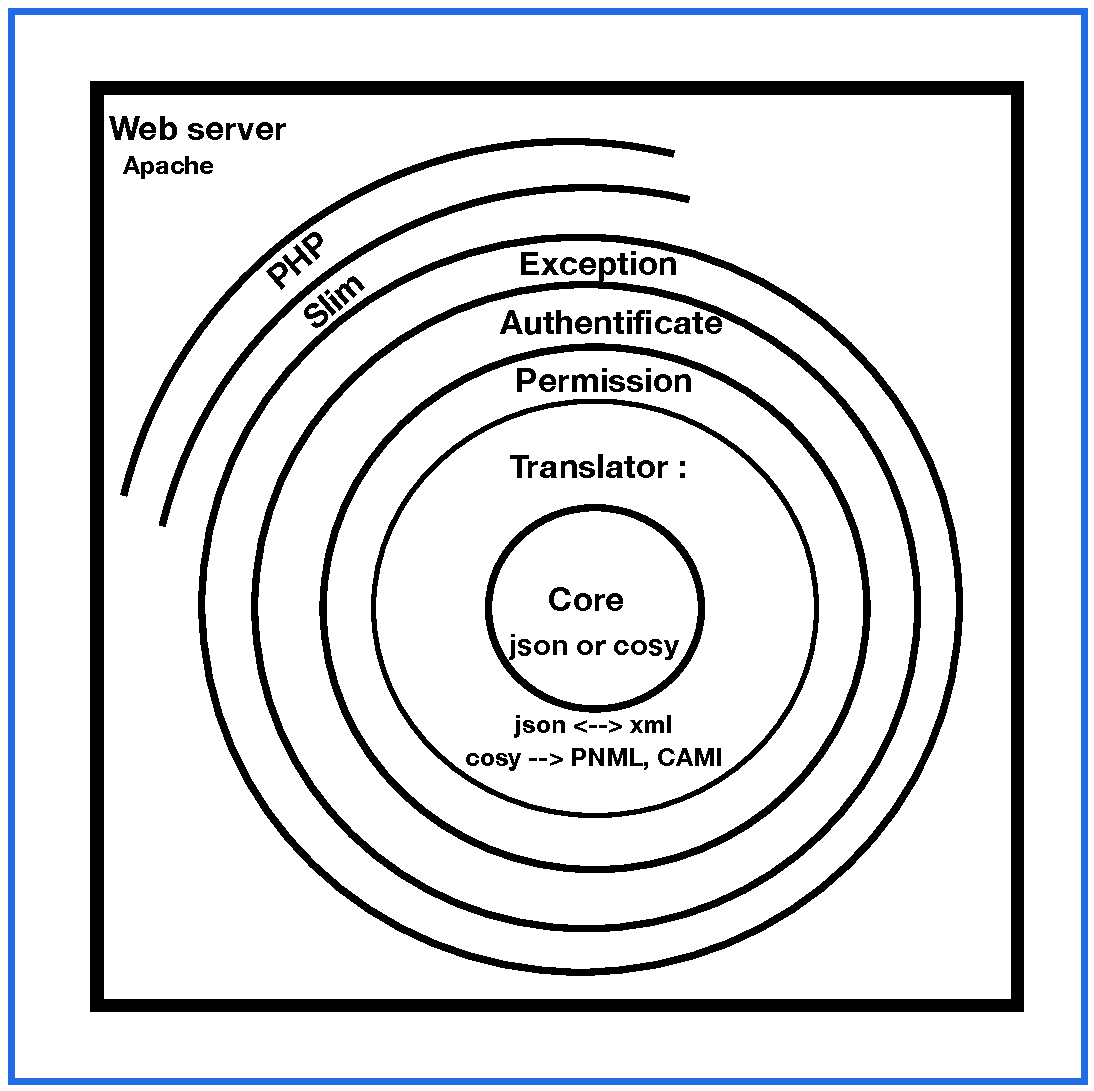
\includegraphics[scale=0.60]{img/server_couches.pdf}
     \caption{Couches du serveur}
\end{figure}

\subsubsection{Module Exception}

Le module exception gère les exceptions produites pendant le traitement des requêtes. Nous distinguons les 
exceptions des cas d'erreurs qui sont directement traités au moment où ils
sont produits. Les exceptions produites dans
le serveur sont causées par des problèmes graves. La plupart du temps, elles proviennent du système de fichiers et sont capturées par cette couche. Nous ne traitons pas ces exceptions car
elles nécessitent une intervention humaine. Pour cela, un message est envoyé à l'administrateur du serveur
avec la description de l'exception qui va pourvoir intervenir. Ce module est réalisé.

\subsubsection{Module Authentication}

Le module Authentication gère l'authentification des utilisateurs. Ainsi, quand la requête arrive à cette couche, son
utilisateur est soumis à l'authentification. Il a été réalisé avec la méthode d'authentification basique de la spécification
du protocole HTTP car les échanges entre les clients et le serveur utilisent le protocole HTTPS qui assure la sécurité
du transport. Ce module est réalisé.

\subsubsection{Module Permission}

Le module Permission gère les droits d'accès aux ressources par des utilisateurs. Ainsi, quand la requête arrive
à cette couche, les droits d'utilisation de l'utilisateur sur la requête sont vérifiés. 

\subsubsection{Module Translation}

Le module Translation gère les conversions de formats vers d'autres formats. Ainsi, quand la requête arrive
à cette couche et qu'il y a lieu de traduction, il traite la traduction. Cette couche ne concerne pas
mon stage et est liée au serveur d'exécution d'outils qui sera réalisé plus tard. Donc, ce module n'est pas réalisé.

\subsubsection{Module Core}

\paragraph{}
Le module Core gère l'accès et la mise à jour des ressources sur le système de fichiers. C'est une bibliothèque de 
fonctions réutilisables par l'ensemble de parties du serveur.

\subsection{Description de l'environnement de développement}

Un environnement de développement a été mis en place pour réaliser le serveur. Notamment :

\begin{itemize}
\item  Un serveur web Apache : c'est un serveur d'application web nécessaire pour le développement 
du serveur.
\item PHP (version 5.4.24) : c'est un langage serveur qui va permettre au serveur apache d'interpréter le code PHP.
\item Un éditeur : sublime text 3 est utilisé (par simple goût du développeur).
\item Outil Git : le code et documents produits sont envoyer vers le dépôt Github de CosyVerif % l'url du dépôt en note de page
\item Box : pour construire un phar du serveur.
\item Composer : va gérer toute les dépendances du projet.
\item PHPUnit : va aider à faire les tests.
\end{itemize}

Le processus d'installation des outils et des dépendances, le processus de tests et la production de documents ont été  automatisé à l'aide d'un script Bash.


\subsection{Tests}

Les tests du serveur se sont basés sur des tests fonctionnels en boîte noire avec comme
intention une couverture complète du code. Ainsi, pour chaque
fonctionnalité, des scénarios et des test sont écris, validés par mes encadrants puis implémentés. Les outils 
PHPUnit, Guzzle et Travis sont utilisés pour faire le test. Ces tests permettent de s'assurer que le serveur 
fonctionne correctement, fonctionnellement. Pour le moment, on a une bonne couverture mais il reste quelques
points à améliorer qui seront faits avant la fin du stage.

\subsection{Bilan}

J'ai réalisé complètement un serveur REST écris en PHP disposant d'un gestionnaire de comptes utilisateurs et d'un 
dépôt de modèles et de formalismes. En plus, le serveur dispose d'une bibliothèque de fonctions permettant 
d'intégrer facilement la partie édition collaborative et la partie exécution d'outils. 

La couverture de code par les tests est bonne mais il reste quelques améliorations à faire et seront réalisées avant la
fin du stage.

\subsection{Perspective}

Il y a des perspectives à court terme qui sont l'amélioration de la couverture de code, l'intégration des parties
serveur d'édition collaboratif de modèles (en cours de réalisation par Alban Linard) et serveur d'exécution d'outils 
et la réalisation d'un script d'installation. Mais aussi des perspectives à moyen terme qui sont l'ajout de la notion de 
classe d'étudiants au dépôt de modèles et de formalismes.


\chapter{Etudes et réalisations de l'interface web}

\paragraph{}
Au début de mon stage a été la conception et la réalisation du serveur de la nouvelle plate-forme de CosyVerif mais
maintenant, il a été étendu par la réalisation d'un client web. Ce client va offrir une interface pour chaque fonctionnalité
du serveur. 

\section{Présentation}

\paragraph{}
Le client est une interface web permettant à des utilisateurs d'interagir avec le serveur. Il propose une interface pour chaque 
fonctionnalités du serveur de la nouvelle plate-forme de CosyVerif. Il permet donc à un utilisateur de :

\begin{itemize}
\item créer son compte utilisateur et s'authentifier,
\item créer, lire et modifier ses ressources (modèles, formalismes, services et exécutions),
\item rechercher ses ressources et/ou autres ressources publiques selon certains critères,
\item mettre à jour son compte,
\item rendre publique ou privé son compte pour autoriser l'accès ou non à tous les utilisateurs en lecture seule,
\item créer un projet pour partager des ressources avec quelques utilisateurs,
\item inviter un utilisateur à un projet,
\item faire une requête pour se joindre à un projet,
\item créer, lire et modifier les ressources (modèles, formalismes, services et exécutions) d'un projet,
\item changer les droits d'un utilisateur,
\item supprimer un utilisateur d'un projet,
\item mettre à jour les informations d'un projet,
\item supprimer un compte ou un projet.
\end{itemize}

\section{Définition de l'architecture}

\paragraph{}
Le client est juste une page web écrit avec des technologies standard HTML, JavaScript et CSS. Il permet d'envoyer des 
requêtes REST (basé sur la spécification du protocole HTTP) au serveur via le framework JQuery. Il est construit avec une
utilisation de templates de HTML5 pour une meilleure réutilisation du code. Les données échangés avec le serveur sont
au format JSON.

\section{Etude technique}

\paragraph{}
Cette partie récence les technologies utilisées

\subsection*{HTML5}

\paragraph{}
HTML (Hypertext Markup Language) est le format de données conçu pour représenter les pages web. Il permet de 
structurer sémantiquement et de mettre en forme le contenu des pages, d’inclure des ressources multimédias dont des 
images, des formulaires de saisie, et des programmes informatiques. Il permet de créer des documents interopérables 
avec des équipements très variés de manière conforme aux exigences de l’accessibilité du web. HTML5 est sa version
évolué qui ajoute des nouvelles fonctionnalités comme description des applications en ligne, d'enrichir les interfaces
utilisateurs avec des contrôles spécifiques : menus, champs associés à des types de données spécifiques, ... Il est le
langage qui s'occupe des aspects statiques de l'interface du client web.


\subsection*{JavaScript}

\paragraph{}
Le langage de programmation pour les aspect dynamique d'une page. Dans un document HTML, il est possible de définir 
des fonctions associé à des événements, et ainsi de modifier l’apparence de l'interface (HTML), d'ajouter de nouveaux 
éléments à la page, de valider les données de formulaires, de faire des requêtes asynchrone au serveur de la plate-forme
de CosyVerif.

\subsection*{CSS}

\paragraph{}
Les styles CSS, pour feuilles de style en cascadent, permettent de définir l’aspect d'une page et de ses éléments par un 
ensemble de propriétés (position, taille, couleurs, bordures, polices, visibilité…), en fonction de certains paramètres 
comme la taille ou la nature du support associé, ou de l'état de ces éléments, si la souris est positionnée sur un élément 
il est par exemple possible de changer son aspect. Par exemple à l'impression d'une page web il est possible de définir 
un style qui permet de cacher les éléments de navigation inutiles sur papiers. Il a permis au client d'avoir une ergonomie
moderne.

\subsection*{jQuery}

\paragraph{}
jQuery est une bibliothèque JavaScript facilitant d'écrire de scripts côté client dans le code HTML des pages web. 
Combiné avec JavaScript, il nous a permis de réaliser les aspects dynamiques du client.

\subsection*{Bootstrap}

\paragraph{}
Bootstrap est un framework qui fournit le placement en grille dynamiquement pour bien disposer les composants d'une
page HTML et  des composants utiles (des composants HTML mise en forme).

\subsection*{Handlebars}

\paragraph{}
Handlebars est un framework qui permet une utilisation simple de templates de HTML5 pour une meilleure réutilisation 
du code. Il a permis de factoriser beaucoup de codes qui sont réutilisés après.

\section{Mise en oeuvre}

\paragraph{}
Le client web a été développé sur une nouvelle base. En effet, tout le code produit est nouveau. Il est réalisé de manière
à être simple et maintenable en utilisant des bibliothèques standards :

\paragraph{Code réutilisable :} des templates ont été réalisés, utilisés, réutilisés. Des futures fonctionnalités 
peuvent réutiliser ces templates. Ils sont réalisés grâce au framework "Handlebars". En plus, cinq fonctions en 
JavaScript-jQuery seulement pour tout le code permettant d'interagir avec le serveur (post, get, post et del, patch).
 
\paragraph{Composants standards :} grâce au framework Bootstrap le client web est écris avec des composants standards
placés en grille dans la page web. En plus, les mêmes composants sont utilisés par l'éditeur web.

\subsection{Exemples d'écran de sortie}

\subsubsection{Interface d'accueil du client web}

\paragraph{}
Sur la page d'accueil, l'utilisateur peut se connecter à son compte utilisateur, créer un compte s'il n'en a pas, chercher
des ressources dont il est autorisé à lire et filtrer le résultat de la recherche par type de ressources (voir figure 3.1)

\newpage

\begin{figure}[h!]
     \centering
     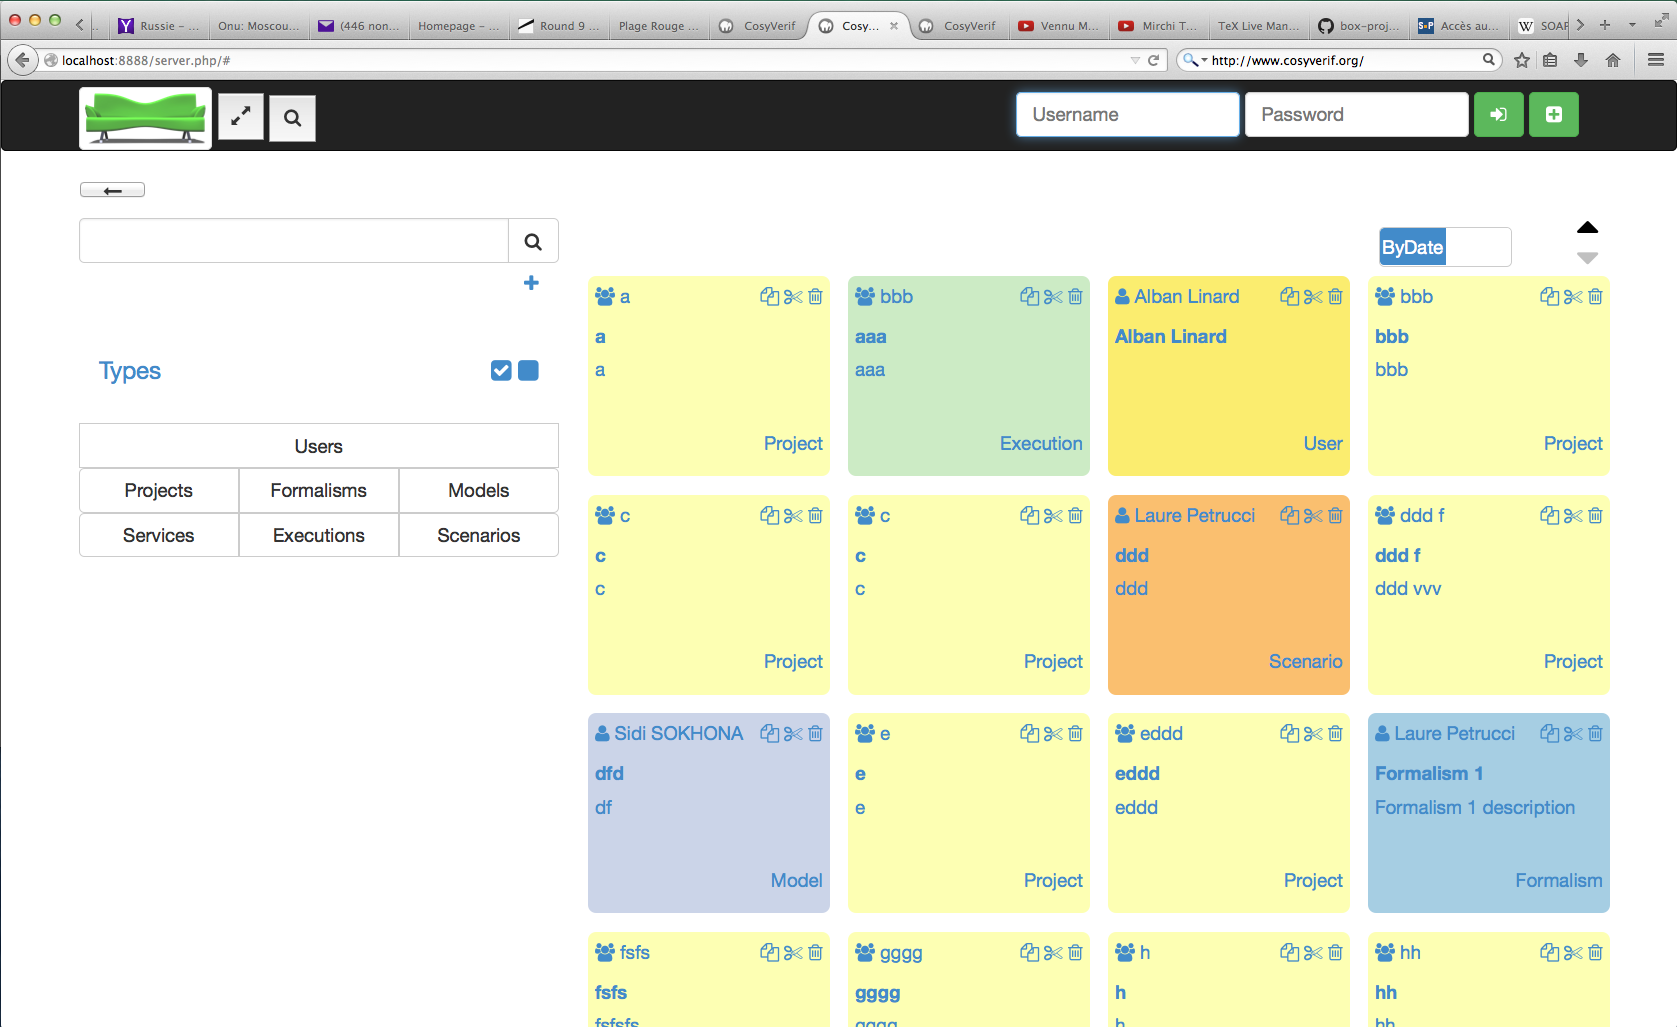
\includegraphics[width=0.8\textwidth] {img/1-ecran-create-user}
     \caption{interface d'accueil}
\end{figure}

\subsubsection{Interface de recherche}

\paragraph{}
La figure suivante (Figure 3.2) représente la page de recherche. Il permet à un utilisateur de faire des recherches.
Il permet à l'utilisateur de choisir de rechercher dans son compte ou dans tout le dépôt, de rechercher par un ou
plusieurs types, par un ou plusieurs projets.
 par
un ou plusieurs types de resources, 

\newpage

\begin{figure}[h!]
     \centering
     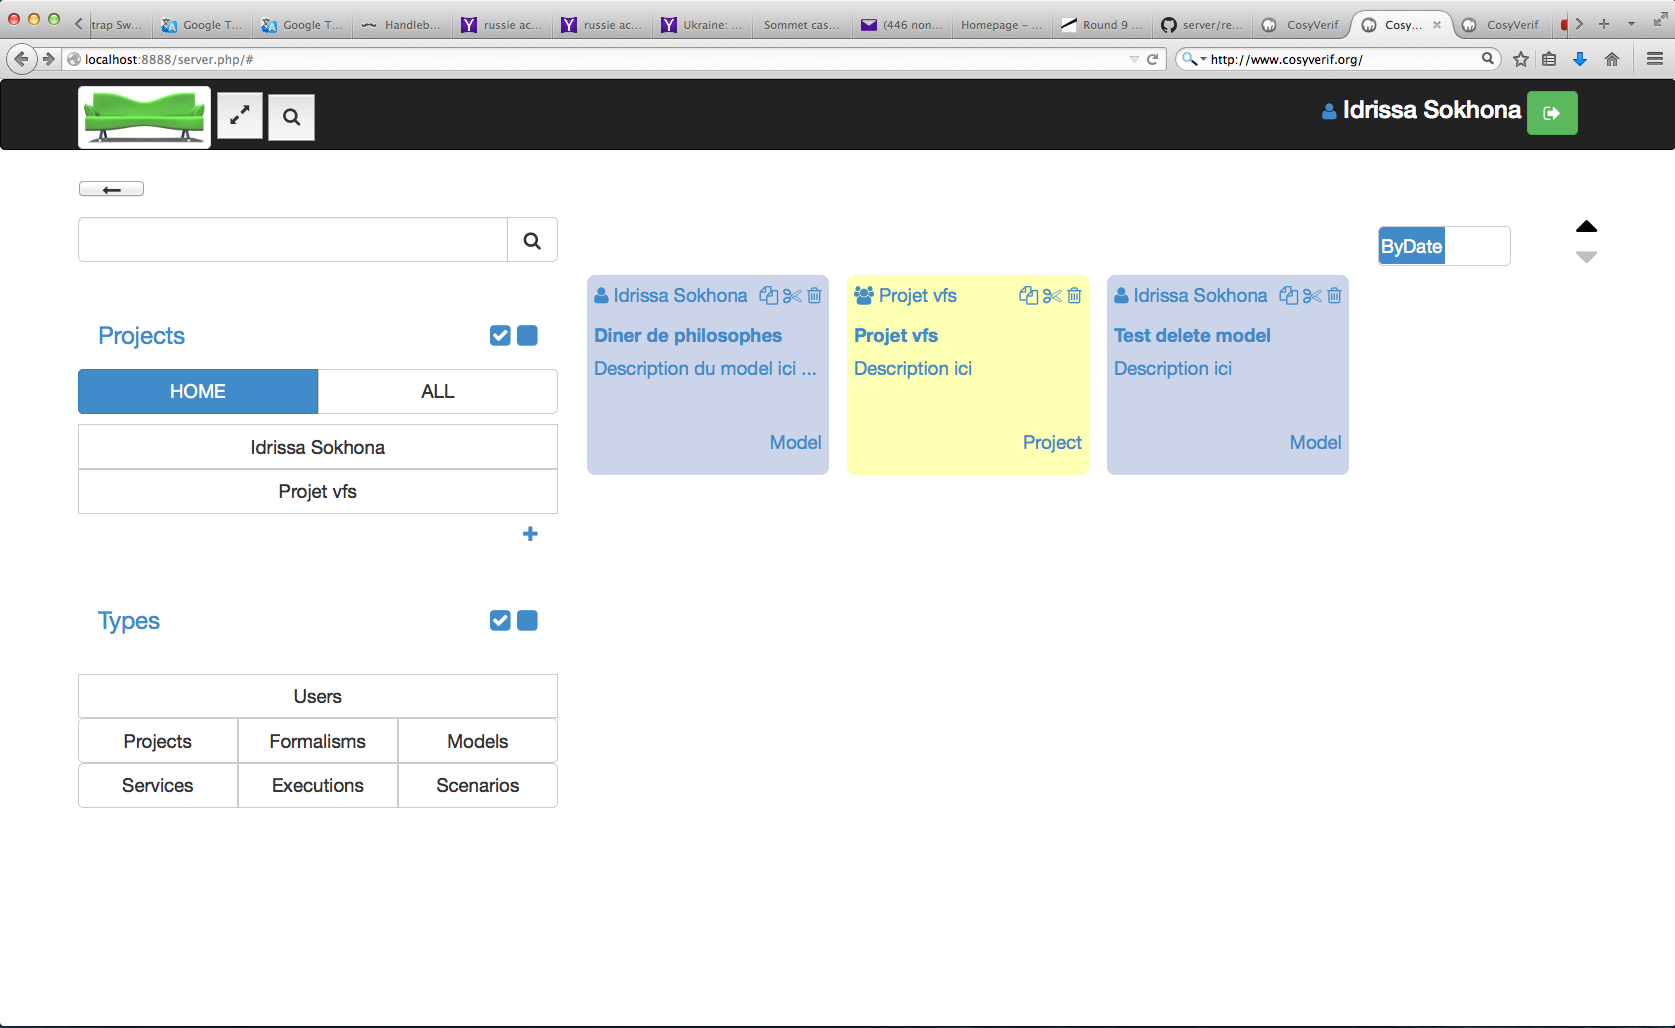
\includegraphics[width=0.8\textwidth] {img/1-ecran-recherche}
     \caption{écran de recherche}
\end{figure}







\subsection{Bilan}
\subsection{Perspective}
classe étudiant : lauré



\chapter*{Conclusion}
\addcontentsline{toc}{chapter}{Conclusion}

L'objectif initial de mon stage de fin d'études était l'élaboration du
nouveau serveur de CosyVerif, permettant entre autres la gestion
d'utilisateurs et servant de dépôt de modèles.
Au cours du stage, il a été étendu pour réaliser un client web interagissant avec le serveur.

La première partie de ce rapport présente le projet dans son environnement organisationnel
(présentation du projet, des laboratoires partenaires, ...)
et contextuel (description de l'existant et des problèmes identifiés sur le
projet)
afin de mieux cerner mes mes objectifs.

La deuxième partie explique la conception et la réalisation du serveur, en définissant son architecture et le protocole de communication
qu'il utilise avec ses clients. Cette partie présente aussi les choix
techniques et leur mise en oeuvre.
Cette aboutit à la réalisation d'un serveur avec les fonctionnalités attendues.

Enfin, la troisième partie décrit la réalisation d'un client web fournissant
une interface pour chaque fonctionnalité du serveur. Cette partie amène à la réalisation d'un client avec une interface moderne basé sur des bibliothèques standards.

Durant tout le stage, j'ai veillé à respecter les objectifs qualité requis.
J'ai eu à proposer des solutions, argumenter mes choix.
Le processus n'a pas été linéaire. En effet, j'ai tenu compte aussi bien des
remarques que des changements de direction proposés par mes encadrants,
la conception n'étant pas figée à mon arrivée.
J'ai ainsi appris à concevoir et développer un système par prototypage et incréments.
Ces techniques sont maintenant couramment utilisées dans le cadre de
développement agiles.

Mon travail a aboutit à deux logiciels fonctionnels : le serveur et le client.
Ceux-ci seront utilisés dans la nouvelle plateforme CosyVerif.

Au cours de ce stage de fin d'études, j'ai eu l'opportunité de mettre en application différentes connaissances acquises 
durant mes études à l'Université Pierre et Marie Curie. Par ailleurs, j'ai
tiré grand bénéfice du stage, aussi bien au niveau technique
qu'au niveau professionnel. En effet, ce stage m'a permis de découvrir beaucoup de technologies et m'a permis de comprendre
différentes facettes pour la réalisation d'un système client / serveur.

Ce stage m'a de plus permis d'affiner ma méthodologie de travail et de 
développer l'esprit de responsabilité, autonomie et rigueur.

\end{document}

%% Exigences du rapport 
 %% Le Rapport de conception doit contenir :
  % - Remerciement (20 mn) 
  % - Sujet du stage (20 mn) (ok)
  % - Introduction (20 mn)
  % - Présentation de CosyVerif (client coloane, server alligator, client clitoris, nouveau server nouveau client) (30 mn)
  % - Présentation de LSV et LIPN (30 mn)
  % - Présentation du nouveau serveur et du dépot de modèles (30 mn)
  % - Développement du serveur et du dépot (Besoins, Architecture-protocole, outils, objectifs-planning (échances)) (30 mn)
  % - Test
  % - Conclusion (20 mn)
  % - Glossaire
  % - Webographie (20 mn)
  % - Annexes (20 mn)


%% Nota bené :
 % Le découpage

% - La structure du rapport, 
% - l'introduction, 
% - la présentation de l'entreprise, 
% - la présentation du sujet, 
% - le découpage de votre travail,
% - un premier chapitre d'étude et/ou de développement, 
% - des éléments de bibliographie doivent déjà exister.

